% ----------------------------------------------------------
% Estrutura do Texto
% ----------------------------------------------------------
\vspace*{1cm}
\chapter{Desenvolvimento} \label{chap:estrutura}

Parte mais importante do artigo. Deve conter a explanação do assunto de maneira organizada e bem delineada. Pode ser dividido em seções e subseções, de acordo com a NBR 6024/2012 \cite[p. 33]{sperandio}

Neste espaço são expostas argumentações às ideias de forma objetiva e, que estejam em consonância com o tema abordado na introdução. O desenvolvimento deve ser fundamentado em referencial teórico.

Tanto a estrutura do texto, quanto a numeração sequencial dos itens, as citações e referência devem seguir as normas da ABNT destinadas a cada caso e conforme estabelecido no Manual de TCC do 
IFPI. O mesmo vale para as ilustrações.

\begin{citacao}
Usar fonte Arial ou Times New Roman, tamanho 10 ou 11, nestes casos: nas citações com mais de três linhas, nas notas de rodapé, na indicação da fonte (autoria) das figuras, quadros e tabelas, bem como nas legendas e nos 
conteúdos dos quadros e das tabelas. Para a citação com mais de três linhas deixar uma linha em branco antes e outra após a citação direta e recuo de 4 cm da margem esquerda. (AUTOR, ano, p. xx).
\end{citacao}

Quando o autor do trabalho científico faz uma transcrição textual (cópia) de parte da obra de outros autores para fundamentar sua produção textual. Quando até 3 linhas é considerada curta e mais de 3 linhas é considerada longa.

\begin{quadro}[htb]

{
\caption{\label{quadro_exemplo}Estilos cognitivos propostos por psicólogos.}
}
 \begin{tabular}{|c|c|c|c|}

 \hline
 \rowcolor[HTML]{D2DFEC} 
 \textbf{01} & \textbf{Amplo/restrito} & \textbf{Preferência por pensar em termos de poucas...} \\
 \hline
 \rowcolor[HTML]{A7BDDE} 
 02 & Analítico/não analítico & Tendência à diversificação entre muitos atributos \\ \hline
 \rowcolor[HTML]{D2DFEC} 
 03 & Disperso/concentrado & Tendência a perder detalhes versus tendência \\ \hline
 \rowcolor[HTML]{A7BDDE}
 04 & Impulsivo & Tendência a reagir rapidamente versus tendência... \\ \hline
 \rowcolor[HTML]{D2DFEC} 
 05 & Convergente/divergente & Pensamento lógico e dedutivo versus pensamento... \\ \hline
 \rowcolor[HTML]{A7BDDE}
 06 & Sequencial/holístico & Preferência por trabalhar em sequência... \\ \hline
 \end{tabular}
 \fonte{\citeonline{willingham2022alunos}.}
  
\end{quadro}



\section{Orientações sobre ilustrações e tabelas}

As tabelas devem apresentar informações tratadas de maneira estatística, de acordo com o Instituto Brasileiro de Geografia e Estatística (IBGE).

Segundo a \citeonline{NBR14724/2011} a tabela é uma forma não discursiva de apresentar informações das quais o dado numérico se destaca como informação central.

Se houver figuras, quadros e/ou tabelas, estas devem ser inseridas no texto e estar devidamente citadas.

\begin{table}[H]
\caption{\label{tabela_exemplo}Exemplo de Tabela}
\centering
\begin{tabular}{c|c|c|c}
\hline
\textbf{Cursos} & \cellcolor[HTML]{C0C0C0}\textbf{Títulos} & \textbf{Exemplares} & \textbf{Percentual} \\ \hline
\rowcolor[HTML]{C0C0C0} 
Matemática & 55 & 383 & \textbf{19\%} \\ \hline
Biologia & \cellcolor[HTML]{C0C0C0}68 & 443 & \textbf{22\%} \\ \hline
\rowcolor[HTML]{C0C0C0} 
Agronomia & 81 & 474 & \textbf{25\%} \\ \hline
Ensino Médio & \cellcolor[HTML]{C0C0C0}145 & 655 & \textbf{34\%} \\ \hline
\multicolumn{1}{r}{Total} & \cellcolor[HTML]{C0C0C0}\textbf{349} & \textbf{1.955} & \textbf{100\%} \\ \hline
\end{tabular}
\end{table}

\section{Orientações sobre as referências}

A fonte das referências deve ser Arial ou Times New Roman, tamanho 12, com espaçamento simples entre as linhas, alinhamento à margem esquerda, sem recuo, com um espaço simples entre cada referência. O título Referências deve ser centralizado na página, grafado em negrito e em maiúsculas.

Para compor cada referência, seguir o que diz a NBR 6023-2018, observando os exemplos de cada tipo de material que a norma apresenta.

\subsection{Observação sobre a lista de referências }

A lista de referências deve conter somente as obras citadas ao longo do texto. Ao montar a lista, observar se a referência realmente foi citada; e vice versa. 

\begin{figure}[h]
\caption{Exemplo de Figura}
\centering
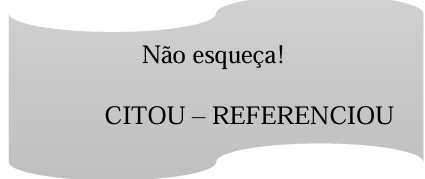
\includegraphics[width=0.5\textwidth]{imagens/ref_.jpg}
\end{figure}

As referências que seguem abaixo da conclusão ou considerações finais são meramente ilustrativas para este template.